\documentclass[12pt, titlepage]{article}

\usepackage{amsmath, mathtools}
\usepackage{amsfonts}
\usepackage{amssymb}
\usepackage{xr}
\externaldocument[ext1-]{../../SRS/CA}
\externaldocument[ext2-]{../../Design/MG/MG}
\externaldocument[ext3-]{../../Design/MIS/MIS}

\usepackage{caption}
\usepackage{pdflscape}
\usepackage{afterpage}
\usepackage{caption}
\usepackage{pbox}
\usepackage{makecell}


\usepackage{booktabs}
\usepackage{tabularx}
\usepackage{hyperref}
\hypersetup{
    colorlinks,
    citecolor=black,
    filecolor=black,
    linkcolor=red,
    urlcolor=blue
}
\usepackage[sort&compress,square,comma,numbers]{natbib}
\newcounter{reqnum} %Requirement Number
\newcommand{\famname}{Lattice Boltzmann Solver} 
\newcounter{testcounter} %Test Number
\newcommand{\athetestcounter}{P\thetestcounter}
%% Comments

\usepackage{color}

\newif\ifcomments\commentstrue

\ifcomments
\newcommand{\authornote}[3]{\textcolor{#1}{[#3 ---#2]}}
\newcommand{\todo}[1]{\textcolor{red}{[TODO: #1]}}
\else
\newcommand{\authornote}[3]{}
\newcommand{\todo}[1]{}
\fi

\newcommand{\wss}[1]{\authornote{blue}{SS}{#1}} 
\newcommand{\plt}[1]{\authornote{magenta}{TPLT}{#1}} %For explanation of the template
\newcommand{\an}[1]{\authornote{cyan}{Author}{#1}}

%% Common Parts

\newcommand{\progname}{ProgName} % PUT YOUR PROGRAM NAME HERE %Every program
                                % should have a name


\begin{document}

\title{System Verification and Validation Plan for \famname} 
\author{Peter Michalski}
\date{\today}
	
\maketitle

\pagenumbering{roman}

\section{Revision History}

\begin{tabularx}{\textwidth}{p{4cm}p{2cm}X}
\toprule {\bf Date} & {\bf Version} & {\bf Notes}\\
\midrule
Oct. 28, 2019 & 1.0 & Initial Document\\
\bottomrule
\end{tabularx}

\newpage

\tableofcontents

\newpage

\listoftables

\listoffigures

\newpage

\section{Symbols, Abbreviations and Acronyms}

\subsection{Abbreviations and Acronyms}

\renewcommand{\arraystretch}{1.2}
\begin{tabular}{l l} 
  \toprule		
  \textbf{symbol} & \textbf{description}\\
  \midrule 
  1D & One Dimensional\\
  2D & Two Dimensional\\
  A & Assumption\\
  C & Pseudo-Oracle Control Value\\
  CA & Commonality Analysis\\
  I & Individual Parameter Input Values\\
  IDE & Integrated Development Environment\\
  LBM & Lattice Boltzmann Method\\
  LBS & Lattice Boltzmann Solvers\\
  MG & Module Guide\\
  MIS & Module Interface Specification\\
  MTBF & Mean Time Between Failures\\
  NAN & Not A Number\\
  NFR & Non-Functional Requirement\\
  O & Program Output\\
  OTS & Off The Shelf\\
  P & Program\\
  R & Functional Requirement\\
  SRS & Software Requirement Specification\\
  V & Set of All Inputs\\
  VnV & Verification and Validation\\
  \bottomrule
\end{tabular}\\

\newpage

\subsection{Symbols}

\renewcommand{\arraystretch}{1.2}
\begin{tabular}{l l} 
  \toprule		
  \textbf{symbol} & \textbf{description}\\
  \midrule 
  $\mathrm{D}$ & Signifies the Dimension Component of Lattice Model\\
  $D_{l}$ & Length of the Domain\\
  $D_{w}$ & Width of the Domain\\
  $\mathrm{e_{fac}}$ & Velocity of Scheme\\
  $\mathrm{e_{max}}$ & Max Velocity in the Middle of Channel\\
  $\mathrm{e_{sch}}$ & Velocity Slowdown Factor\\
  $\eta_b$ & Bulk Viscosity \\
  $\eta_s$ & Shear Viscosity \\
  $\mathbb{N}$ & natural numbers\\
  $\mathrm{Q}$ & Signifies Number of Velocity Directions of Lattice Model\\
  $R$ & Radius of Cylinder\\
  $Re$ & Reynolds Number\\
  $\rho$ & Density \\
  $S$ & Spatial Step - Number of Spatial Subsections\\
  $t$ & Time \\
  $X_{max}$ & Highest X-Axis Interval of Boundary\\
  $X_{min}$ & Lowest X-Axis Interval of Boundary\\
  $Y_{max}$ & Highest Y-Axis Interval of Boundary\\
  $Y_{min}$ & Lowest Y-Axis Interval of Boundary\\
  \bottomrule
\end{tabular}\\

\newpage

\pagenumbering{arabic}

\noindent This document covers the system Verification and Validation (VnV) of
\famname . Functional and non-functional requirements, as found in Section
\ref{objectives} and retrieved from the Commonality Analysis (CA)
(\citet{LBM_CA_PM}), will be tested. The document will outline the general
information of the system in Section \ref{generalinfo}, which will be followed
by a testing plan in Section \ref{testplan}. Finally, individual tests will be
described in Section \ref{systest}.

\section{General Information} \label{generalinfo}
This section of the document will begin with a summary of {\famname}, objectives and a listing of relevant documents.
%\wss{There should generally be text between section headings.  In this case a ``roadmap'' of the contents of this section would be helpful.}

\subsection{Summary}

The software being tested is \famname. This software reads inputs from a file,
and calculates outputs using Lattice Boltzmann Methods (LBM). The software
outputs the results to the screen, to a file, and/or to memory.

\noindent {\famname} can model many fluid dynamics problems, including
Poiseuille Flow and Von Karman Vortex Street. Both of these problems will be
used in our functional test cases, as the results of {\famname} can be compared
to the results of the pseudo-oracle pyLBM (\citet{pylbmcode}).

\subsection{Objectives} \label{objectives}

The intended objective of this plan is to verify that functional requirements
and non-functional requirements (NFR), as found in Section \ref{ext1-CAFRS} and Section \ref{ext1-CANFRS} of the CA titled Lattice Boltzmann Solvers (\citet{LBM_CA_PM}), have been met. %\wss{Copying and pasting your requirements here from your CA is a maintenance problem.  It will be difficult to keep the two documents in sync.  You can just reference the document where the requirements are, without repeating them.  You can even use cross-referencing to reference labels in another document.  That is why the original Blank Project Template has make files, so that running make will update the references between documents.}

%\noindent The functional requirements are:
%\noindent \begin{itemize}
%\item[R\refstepcounter{reqnum}\thereqnum \label{R_Inputs}:] The system shall read a set of input fluid parameters.

%\item[R\refstepcounter{reqnum}\thereqnum \label{R_ModelInputs}:] The system shall allow the user to select from a set of model and velocity direction parameters.  %\wss{This requirement has to be more specific.  What are the velocity and direction parameters?  I feel like you summarized them in your CA.} %Yes they are summarized in the CA. I have temporarily commented out this section in order to keep your comments and respond to them.

%\item[R\refstepcounter{reqnum}\thereqnum \label{R_CheckInputs}:] The system shall verify that the inputs fall within the allowable parameters of variation. %\wss{Where is this documented?  There should be a pointer to this information.  Again, I think this is in your CA, which is another argument for not reproducing the requirements here.} %The CA has this documented.

%\item[R\refstepcounter{reqnum}\thereqnum \label{R_Instantiate}:] The system shall instantiate required data types and structures for the selected model.

%\item[R\refstepcounter{reqnum}\thereqnum \label{R_CoefficientWeights}:] The system shall import the relevant coefficient weights for the selected model.

%\item[R\refstepcounter{reqnum}\thereqnum \label{R_Calculate}:] The system shall calculate and store the predicted fluid parameters, iterating through streaming and collision processes over the desired model time.

%\item[R\refstepcounter{reqnum}\thereqnum \label{R_Output}:] The system shall output the results of the calculations in a manner consistent with the decisions made regarding variabilities.

%\end{itemize}

%\noindent The NFRs are:

%\begin{enumerate}
%\item Correctness: The output results will be compared to the results taken from of a sample of OTS solutions. %\wss{NFRs should not mention modules.  They should be about the software as a whole.  You might want to specify correctness as the comparison between the OTS solution and your solution running the test cases defined in this document.} %This has been addressed in the CA
%\item Maintainability: The system shall be documented with a CA, VnV plan, MG (Module Guide), MIS (Module Interface Specification), and User Guide.
  %\wss{This is how you intend to achieve maintainability, not how maintainability is defined.} %This is changed in the CA
%\item Performance: The system shall be able to run modules faster than a sample OTS implementation.
%\item Portability: The system shall be able to run on macOS, Windows, and Linux operating systems.
%\item Reliability: The mean time between failures (MTBF) will be longer than the average MTBF of a sample of the OTS solutions.
%\item Reusability: Individual modules of the system can be removed and reused in other systems.
%\item Robustness: The system shall behave reasonably in circumstances that were not anticipated in the requirements specification \cite{ghezzi1991fundamentals}.
%\item Scalability: The system must be able to support additional computational models.
%\item Understandability: New users must easily understand which LBM models are available in {\famname}.
%\item Usability: Users will find the system easy to use.
%\end{enumerate}

\subsection{Relevant Documentation}

The CA of {\famname} can be found in (\citet{LBM_CA_PM}).The link to Section \ref{ext1-CAREVHISTORY} navigates to the document, beginning with the revision history. The MG can be found in (\citet{LBM_MG_PM}). The link to Section \ref{ext2-MGREVHISTORY} navigates to the document, beginning with the revision history. The MIS can be found in (\citet{LBM_MIS_PM}). The link to Section \ref{ext3-MISREVHISTORY} navigates to the document, beginning with the revision history.
	%\wss{Although they aren't written yet, you should fake this as if the design documentation is written.  The documentation is also relevant for this problem.}
\newpage

\section{Plan}
\label{testplan}	
\subsection{Verification and Validation Team}

This VnV plan will be conducted by Peter Michalski and several
classmates, including the primary reviewer Ao Dong, and secondary reviewers Sasha Soraine, Bo Cao, and Zhi Zhang. %\wss{Be specific and name the relevant classmates here.}

\subsection{CA Verification Plan}

The CA of {\famname} shall be verified in the following ways:

\begin{enumerate}
\item Feedback: Classmates, including all primary and secondary reviewers listed above, shall provide feedback on GitHub. They shall read the document and provide insight on how to improve the documents and {\famname}. %\wss{Are you going to be more specific?  Is this task directed feedback, or just ``read the document'' and tell me what you think?  Who specifically is going to review the document?}
\item Initial Review: The document shall be manually reviewed by the author
  using the SRS checklist upon its initial creation, as found in the CAS741
  GitLab repository (\citet{CAS741_SRS_checklist}). %\wss{Good!}
\item Second Review: The document shall be manually reviewed by the author using
  the SRS checklist after VnV completion, as found in the CAS741 GitLab
  repository (\citet{CAS741_SRS_checklist}). %\wss{Good!}
\item Final Review: The document shall be manually reviewed by the author using
  the SRS checklist after MG and MIS development, as found in the CAS741
  repository (\citet{CAS741_SRS_checklist}). %\wss{Great!}
\end{enumerate}

\subsection{Design Verification Plan}

The design shall be verified by ensuring that functional requirements and NFRs
are tested, as listed in Section \ref{objectives}.

\noindent The system functional requirements shall be tested first, as outlined
in \ref{testfr}. This will be followed by reviewing the NFRs as outlined in
\ref{nfrtest}.

\subsection{Implementation Verification Plan}
  
\noindent The implementation shall be verified in the following ways:

\begin{enumerate}
\item Code Walkthrough - Author: Module unit code shall be inspected for
  functional errors by the author immediately after MIS document version 1.0 is
  developed. A rubber duck debugging method will be followed. Any defects shall
  be immediately fixed. This plan is described in Section 5.1 of the document
  Unit Verification and Validation Plan for Lattice Boltzmann Solver
  (\citet{LBM_UVNV_PM}).
\item Code Walkthrough - Peer: Module unit code shall be inspected for
  functional errors by Ao Dong after MIS document version 1.0 is submitted on
  GitHub. Defects shall be noted in GitHub using issue creation. This plan is
  described in Section 5.1 of the document Unit Verification and Validation Plan
  for Lattice Boltzmann Solver (\citet{LBM_UVNV_PM}).
\item Dynamic Unit Tests - Author: Dynamic unit test will be carried out, as
  listed in Section 5.1 of the document Unit Verification and Validation Plan
  for Lattice Boltzmann Solver (\citet{LBM_UVNV_PM}).
\item System Tests: System tests will be carried out as listed in Section
  \ref{systest}. The author shall conduct the tests of the functional
  requirements. Tests of the NFRs shall be conducted by those listed in the
  outline of each test.
\end{enumerate}

\subsection{Software Validation Plan}

{\famname} does not have a validation step. Validation is related to comparing the outputs of models to experimental values. {\famname} is simply concerned that its solution is correct mathematically.

%\wss{You do not actually have a validation step.  You should explain in this section that validation is related to comparing the outputs of models to experimental values.  Your software doesn't care whether the models agree with reality, only that they the solutions are correct mathematically.}

~\newpage	 

\section{System Test Description} \label{systest}

\subsection{Tests for Functional Requirements}

\label{testfr}

The subsections below are designed to cover several of the functional
requirements of the system. Subsection \ref{frinput} will cover R1 and
R3. Subsections \ref{frvkvs} and \ref{frpf} will cover R1, R2, R3, R4, R5, R6,
and R7, and will test out the input vales at their allowable edges.

\subsubsection{Input}
\label{frinput}
		
\paragraph{Input Reading}

\begin{enumerate}

\item{input-reading-id\refstepcounter{testcounter}\thetestcounter
    A \label{inputreadingtest}}

  Control: Program (P) reading of input values (V) from a file.
				
  Initial State: input.txt file is in the Input directory. %\wss{If the initial state is no input file, then wouldn't this test fail to generate output?  I would think you would get an exception if the file does not exist?}
					
  Input: A comma delimited text file, with inputs marked in the manner outlined
  in the User Guide (\citet{LBM_UserGuide_PM}).

  The input values for this test will be:

  $Re$: 500\\ 
  $t$: 75\\
  $\rho$: 1.0\\
  $\eta_b$: 1.e-3\\
  $X_{min}$ = 0.\\
  $X_{max}$ = 3.\\
  $Y_{min}$ = 0.\\
  $Y_{max}$ = 1.\\
  $R$ = 0.05\\
  $\mathrm{e_{sch}}$ = 1.\\
  $\mathrm{e_{fac}}$ = 20\\
  $\mathrm{e_{max}}$ = 0.1\\
  $S$ = 64\\
  $\mathrm{D}$ = 2\\
  $\mathrm{Q}$ = 9\\
  $D_{l}$ = 2\\
  $D_{w}$ = 1\\

					
Output: All inputs printed to the screen as output (O).\\
Outputs printed to the screen:\\
$Re$: 500\\
$t$: 75\\
$\rho$: 1.0\\
$\eta_b$: 1.e-3\\
$X_{min}$ = 0.\\
$X_{max}$ = 3.\\
$Y_{min}$ = 0.\\
$Y_{max}$ = 1.\\
$R$ = 0.05\\
$\mathrm{e_{sch}}$ = 1.\\
$\mathrm{e_{fac}}$ = 20\\
$\mathrm{e_{max}}$ = 0.1\\
$S$ = 64\\
$\mathrm{D}$ = 2\\
$\mathrm{Q}$ = 9\\
$D_{l}$ = 2\\
$D_{w}$ = 1\\

Test Case Derivation: P(V) is correct if P:V -$>$ O and O = V\\

The result required for the test to pass is the successful printing of all input
values to the screen. This test satisfies R1.\\
					
How test will be performed: 

\begin{enumerate}
\item Outside of the system, the input parameter values will be written to a
  comma delimited text file titled input.txt, as outlined in the User Guide.
\item The file will be placed into the Input directory, under the home directory
  of the project.
\item {\famname} will be run.
\item If successful, The system will output the input parameters to the screen.
\end{enumerate}

\item{input-reading-id\ref{inputreadingtest}B\\}

Control: Program (P) reading of input values (V) from a file.\\

Initial State: input.txt file is in the Input directory.\\

Input: A comma delimited text file with the following input:\\
ccQseHfFspBLAYZjCGZtJYMAdeAc

Output: An error message of ``cannot read file" should be shown.\\

Test Case Derivation: P(V) is correct if P:V -$>$ Error Message \\

The result required for the test to pass is the successful printing of the error message. This test satisfies R1.\\

How test will be performed: 

\begin{enumerate}
\item Outside of the system, the input parameter value will be written to a
  comma delimited text file titled input.txt, as outlined in the User Guide.
\item The file will be placed into the Input directory, under the home directory
  of the project.
\item {\famname} will be run.
\item If successful, the system will output an error message to the screen.
\end{enumerate}

\end{enumerate}
			
\paragraph{Input Bounds}
This test will be composed of two parts:
\begin{enumerate}
						
\item{input-bounds-id\refstepcounter{testcounter}\thetestcounter A \label{inputboundstest}}
\item{input-bounds-id\ref{inputboundstest}B\\}

Control: Program (P) testing of high and low input values (V) read from a file.\\
					
Initial State: input.txt file is in the Input directory.\\
					
Input: A comma delimited file, with inputs marked in the manner outlined in the
User Guide (\citet{LBM_UserGuide_PM}).\\The input values for this test will
be:\\

\begin{table}[!h]
	\begin{center}
		\begin{tabular}{| c | c | c |}
			\hline
			Input & id2A & id2B \\
			\hline
			$Re$ & 50000 & -500000 \\
			\hline
			$t$ & 0& 0\\
			\hline
			$\rho$ & 15& -15\\
			\hline
			$\eta_b$ & 100& -100\\
			\hline
			$\eta_s$ & 30000& -30000\\
			\hline
			$X_{min}$ & 0.& 0.\\
			\hline
			$X_{max}$ & 3.& 3.\\
			\hline
			$Y_{min}$ & 0.& 0.\\
			\hline
			$Y_{max}$ & 1.& 1.\\
			\hline
			$R$ & 0.05& 0.05\\
			\hline
			$\mathrm{e_{sch}}$ & 1.& 1.\\
			\hline
			$\mathrm{e_{fac}}$ & 20& 20\\
			\hline
			$\mathrm{e_{max}}$ & 0.1& 0.1\\
			\hline
			$S$ & 64& 64\\
			\hline
			$\mathrm{D}$ & 2& 2\\
			\hline
			$\mathrm{Q}$ & 9& 9\\
			\hline
			$D_{l}$ & 2& 2\\
			\hline
			$D_{w}$ & 1& 1\\
			\hline
		\end{tabular}
		\caption{Input Bounds Test Inputs}
	\end{center}
\end{table}
	
Output: A descriptive failure message printed to the screen as seen below, or on the command line depending on how the system is run. In
the below figure, X will contain all parameter names that are out of bounds. In
both tests that will include $Re$, $t$, $\rho$, $\eta_b$, and $\eta_s$.

\begin{figure}[h!]
\begin{center}
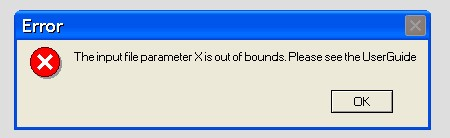
\includegraphics[width=0.6\textwidth]{errorMessage.jpeg}
\caption{Input out of Bounds}
\label{Fig_InputError}
\end{center}
\end{figure}

Test Case Derivation: 
I (individual inputs) are an element of V. P(V) is incorrect if P:V and at least
one I is out of bounds as per Table \ref{table:inputdatabounds}: Input Data
Bounds. This test satisfies R3.\\
					
How test will be performed: 

\begin{enumerate}
\item Outside of the system, the input values will be written to a comma
  delimited text file titled input.txt, as outlined in the User Guide
  (\citet{LBM_UserGuide_PM}).
\item The file will be placed into the Input directory, under the home directory
  of the project.
\item {\famname} will be run.
\item If the test is successful, the system will output a descriptive error message, as seen above, to the screen.\\

\end{enumerate}

\end{enumerate}

%\wss{The previous few tests are a bit repetitive.  I like the idea of testing that the input checks are working, but you could likely summarize the different tests cases in a table.  Give the outline as above for one test case, but then substitute in a reference to the table and explain how the table provides x number of additional tests.  You can still give each of the tests an identifying label, but the label would be in the table.}

~\newpage

\subsubsection{Von Karman Vortex Street}
\label{frvkvs}
		
\paragraph{Dynamic Testing - Manual:}
\paragraph{} These dynamic tests will compare {\famname} output with output from
the pseudo-oracle myLBM (\citet{pylbmcode}). The pseudo-oracle will have the
same inputs as {\famname} for each test. The difference in output between {\famname} and the pseudo-oracle will be compared and noted. %\wss{Rather than an allowed error, we might be better off simply summarizing the calculated error.  Even if there is an allowed error, a report of the actual error values is more useful information than simply PASS/FAIL.}

\begin{enumerate}

\item{tutorial-test-id\refstepcounter{testcounter}\thetestcounter \\}

Control: Program (P) module execution using inputs (V), and expecting output (O)
to match a control value (C).\\
					
Initial State: input.txt file is in the Input directory. %\wss{Again, this seems like an odd initial state.}\\
					
Input: A comma delimited file, with inputs marked in the manner outlined in the
User Guide (\citet{LBM_UserGuide_PM}).\\The input values for this test will
be:\\
$Re$: 500\\
$t$: 75\\
$\rho$: 1.0\\
$\eta_b$: 1.e-3\\
$X_{min}$ = 0.\\
$X_{max}$ = 3.\\
$Y_{min}$ = 0.\\
$Y_{max}$ = 1.\\
$R$ = 0.05\\
$\mathrm{e_{sch}}$ = 1.\\
$\mathrm{e_{fac}}$ = 20\\
$S$ = 64\\
$\mathrm{D}$ = 2\\
$\mathrm{Q}$ = 9\\

\wss{It is great that you will be using a pseudo-oracle.  However, it would be
  nice to explain what the test inputs mean.  How would a scientist explain the
  test you are running?  What is the physics of the test?  I haven't checked,
  but I would guess that your pyl reference would explain the test cases more
  than just listing numbers?}

Output: Vorticity vector values printed to the screen. \\

Test Case Derivation: This case is a comparison with the pseudo-oracle
pyLBM. The output vector values (C) of this test for pyLBM can be found in the
file id3output.txt located in the OracleOutput folder. The output values of {\famname} will be compared to the pseudo-oracle output values. %\wss{All of your tests that compare to average error should instead be written to output the error values.  I would also like to see your specific relative error calculation formulae for each test case where you mention error.}

How test will be performed:

\begin{enumerate}
\item The Von Karman Vortex Street module shall be modified by the author to
  print the vorticity vector as output.
\item Outside of the system, the input parameter values will be written to a
  comma delimited text file titled input.txt, as outlined in the User Guide.
\item The file will be placed into the Input directory, under the home directory
  of the project.
\item The module for Von Karman Vortex Street will be selected to run.
\item Upon completion of the module, the output values of the vorticity vector
  will be compared to the vorticity vector values from pyLBM - comparison will
  be done per cell. Comparisons can be done manually using Excel, or through a
  script.
\end{enumerate}

\wss{This shouldn't really be a manual test.  Everything described above can be
  done algorithmically.  You can automate this test.  You will need to go
  further to define the mathematical equation for error, but you would still
  need to do this for the manual version.  As part of your development process,
  I could certainly see you doing the test manually the first time, to help
  understand how the pieces fit together.  Once you understand though, the
  target should be automation.  This same comment about changing your manual
  tests to automated tests applies for your other proposed tests as well.}

\item{Reynolds-Rel-Error-test-id\refstepcounter{testcounter}\thetestcounter \\}

Control: Program (P) module execution using inputs (V) with varying $Re$
parameter (I), and observing the variance of the output (O) when compared to a control value (C).  %\wss{If all of the tests are the same except for the value of $Re$, then you could again use a table to summarize the different test cases.}
				
					
Initial State: input.txt file is in the Input directory.\\
					
Input: A comma delimited file, with inputs marked in the manner outlined in the User Guide (\citet{LBM_UserGuide_PM}).\\The input values for each of the iterations of this test will be:\\

\begin{table}[!h]
	\begin{center}
		\begin{tabular}{| c | c | c | c | c | c |}
			\hline
			Input & Iteration 1 & Iteration 2 & Iteration 3 & Iteration 4 & Iteration 5 \\
			\hline
			$Re$ & 500 & 1500 & 2500 & 5000 & 7500 \\
			\hline
			$t$ & 75& 75& 75& 75& 75\\
			\hline
			$\rho$ & 1.0& 1.0& 1.0& 1.0& 1.0\\
			\hline
			$\eta_b$ & 1.e-3& 1.e-3& 1.e-3& 1.e-3& 1.e-3\\
			\hline
			$X_{min}$ & 0.& 0.& 0.& 0.& 0.\\
			\hline
			$X_{max}$ & 3.& 3.& 3.& 3.& 3.\\
			\hline
			$Y_{min}$ & 0.& 0.& 0.& 0.& 0.\\
			\hline
			$Y_{max}$ & 1.& 1.& 1.& 1.& 1.\\
			\hline
			$R$ & 0.05& 0.05& 0.05& 0.05& 0.05\\
			\hline
			$\mathrm{e_{sch}}$ & 1.& 1.& 1.& 1.& 1.\\
			\hline
			$\mathrm{e_{fac}}$ & 20& 20& 20& 20& 20\\
			\hline
			$S$ & 64& 64& 64& 64& 64\\
			\hline
			$\mathrm{D}$ & 2& 2& 2& 2& 2\\
			\hline
			$\mathrm{Q}$ & 9& 9& 9& 9& 9\\
			\hline
		\end{tabular}
		\caption{Reynolds Test Inputs}
	\end{center}
\end{table} 

Output: In each iteration we will have vorticity vector values printed to the screen.\\

Test Case Derivation: This case is a comparison with the pseudo-oracle
pyLBM. The C values of this test for pyLBM can be found in the files
id4\_1\_output.txt, id4\_2\_output.txt, id4\_3\_output.txt, id4\_4\_output.txt, and id4\_5\_output.txt located in the OracleOutput folder. The files hold the C values for iterations 1 to 5 respectively. Each iteration will compare its output to its respective C counterpart. The intent is to discover how changes in $Re$ affect correctness. This may be helpful in improving correctness of the implementation.\\

How test will be performed: 

\begin{enumerate}
\item The Von Karman Vortex Street module shall be modified by the author to
  print the vorticity vector as output.
\item Outside of the system, the input parameter values will be written to a
  comma delimited text file titled input.txt, as outlined in the User Guide.
\item The file will be placed into the Input directory, under the home directory
  of the project.
\item The module for Von Karman Vortex Street will be selected to run.
\item Upon completion of the module, the output values of the vorticity vector
  will be compared to the vorticity vector values from pyLBM - comparison will
  be done per cell. Comparisons can be done manually using Excel, or through a
  script.
\item Steps (a) - (e) will be repeated for each test iteration.
\item The output value of each iteration will be compared to the pseudo-oracle value.
\end{enumerate}
					
\item{laminar-test-id\refstepcounter{testcounter}\thetestcounter \\}

Control: Program (P) module execution using inputs (V), and expecting output (O)
to match a control value (C).\\
					
Initial State: input.txt file is in the Input directory.\\
					
A comma delimited file, with inputs marked in the manner outlined in the User
Guide (\citet{LBM_UserGuide_PM}).\\The input values for this test will be:\\
$Re$: 0.0001\\
$t$: 75\\
$\rho$: 1.0\\
$\eta_b$: 1.e-3\\
$X_{min}$ = 0.\\
$X_{max}$ = 3.\\
$Y_{min}$ = 0.\\
$Y_{max}$ = 1.\\
$R$ = 0.05\\
$\mathrm{e_{sch}}$ = 1.\\
$\mathrm{e_{fac}}$ = 20\\
$S$ = 64\\
$\mathrm{D}$ = 2\\
$\mathrm{Q}$ = 9\\
					
Output: Vorticity vector values printed to the screen.\\

Test Case Derivation: This case is a comparison with the pseudo-oracle
pyLBM. The C values of this test for pyLBM can be found in the file
id5output.txt located in the OracleOutput folder. The output values of {\famname} will be compared to the pseudo-oracle output values.\\

This test covers a very small Reynolds number representing laminar flow.\\

How test will be performed: 

\begin{enumerate}
\item The Von Karman Vortex Street module shall be modified by the author to
  print the vorticity vector as output.
\item Outside of the system, the input parameter values will be written to a
  comma delimited text file titled input.txt, as outlined in the User Guide.
\item The file will be placed into the Input directory, under the home directory
  of the project.
\item The module for Von Karman Vortex Street will be selected to run.
\item Upon completion of the module, the output values of the vorticity vector
  will be compared to the vorticity vector values from pyLBM - comparison will
  be done per cell. Comparisons can be done manually using Excel, or through a
  script.
\end{enumerate}

\item{turbulent-test-id\refstepcounter{testcounter}\thetestcounter \\}

Control: Program (P) module execution using inputs (V), and expecting output (O)
to match a control value (C).\\
					
Initial State: input.txt file is in the Input directory.\\
					
A comma delimited file, with inputs marked in the manner outlined in the User
Guide (\citet{LBM_UserGuide_PM}).\\The input values for this test will be:\\
$Re$: 50000\\
$t$: 75\\
$\rho$: 1.0\\
$\eta_b$: 1.e-3\\
$X_{min}$ = 0.\\
$X_{max}$ = 3.\\
$Y_{min}$ = 0.\\
$Y_{max}$ = 1.\\
$R$ = 0.05\\
$\mathrm{e_{sch}}$ = 1.\\
$\mathrm{e_{fac}}$ = 20\\
$S$ = 64\\
$\mathrm{D}$ = 2\\
$\mathrm{Q}$ = 9\\

Output: Vorticity vector values printed to the screen. \\

Test Case Derivation: This case is a comparison with the pseudo-oracle
pyLBM. The C values of this test for pyLBM can be found in the file
id6output.txt located in the OracleOutput folder. The output values of {\famname} will be compared to the pseudo-oracle output values.

This test covers a very large Reynolds number representing very turbulent flow.\\	
					
How test will be performed: 

\begin{enumerate}
\item The Von Karman Vortex Street module shall be modified by the author to
  print the vorticity vector as output.
\item Outside of the system, the input parameter values will be written to a
  comma delimited text file titled input.txt, as outlined in the User Guide.
\item The file will be placed into the Input directory, under the home directory of the project.
\item The module for Von Karman Vortex Street will be selected to run.
\item Upon completion of the module, the output values of the vorticity vector
  will be compared to the vorticity vector values from pyLBM - comparison will
  be done per cell. Comparisons can be done manually using Excel, or through a
  script.
\end{enumerate}

\item{low-density-test-id\refstepcounter{testcounter}\thetestcounter \\}

Control: Program (P) module execution using inputs (V), and expecting output (O)
to match a control value (C).\\
					
Initial State: input.txt file is in the Input directory.\\
					
A comma delimited file, with inputs marked in the manner outlined in the User
Guide (\citet{LBM_UserGuide_PM}).\\The input values for this test will be:\\
$Re$: 500\\
$t$: 75\\
$\rho$: 7.08e-2\\
$\eta_b$: 1.e-3\\
$X_{min}$ = 0.\\
$X_{max}$ = 3.\\
$Y_{min}$ = 0.\\
$Y_{max}$ = 1.\\
$R$ = 0.05\\
$\mathrm{e_{sch}}$ = 1.\\
$\mathrm{e_{fac}}$ = 20\\
$S$ = 64\\
$\mathrm{D}$ = 2\\
$\mathrm{Q}$ = 9\\

Output: Vorticity vector values printed to the screen. \\

Test Case Derivation: This case is a comparison with the pseudo-oracle
pyLBM. The C values of this test for pyLBM can be found in the file
id7output.txt located in the OracleOutput folder. The output values of {\famname} will be compared to the pseudo-oracle output values.\\

This test covers the low bound for density using a density of liquid hydrogen.\\
					
How test will be performed: 

\begin{enumerate}
\item The Von Karman Vortex Street module shall be modified by the author to
  print the vorticity vector as output.
\item Outside of the system, the input parameter values will be written to a
  comma delimited text file titled input.txt, as outlined in the User Guide.
\item The file will be placed into the Input directory, under the home directory of the project.
\item The module for Von Karman Vortex Street will be selected to run.
\item Upon completion of the module, the output values of the vorticity vector
  will be compared to the vorticity vector values from pyLBM - comparison will
  be done per cell. Comparisons can be done manually using Excel, or through a
  script.
\end{enumerate}

\item{high-density-test-id\refstepcounter{testcounter}\thetestcounter \\}

Control: Program (P) module execution using inputs (V), and expecting output (O)
to match a control value (C).\\

Initial State: input.txt file is in the Input directory.\\
					
A comma delimited file, with inputs marked in the manner outlined in the User
Guide (\citet{LBM_UserGuide_PM}).\\The input values for this test will be:\\
$Re$: 500\\
$t$: 75\\
$\rho$: 13.6\\
$\eta_b$: 1.e-3\\
$X_{min}$ = 0.\\
$X_{max}$ = 3.\\
$Y_{min}$ = 0.\\
$Y_{max}$ = 1.\\
$R$ = 0.05\\
$\mathrm{e_{sch}}$ = 1.\\
$\mathrm{e_{fac}}$ = 20\\
$S$ = 64\\
$\mathrm{D}$ = 2\\
$\mathrm{Q}$ = 9\\

Output: Vorticity vector values printed to the screen. \\

Test Case Derivation: This case is a comparison with the pseudo-oracle
pyLBM. The C values of this test for pyLBM can be found in the file
id8output.txt located in the OracleOutput folder. The output values of {\famname} will be compared to the pseudo-oracle output values.\\

This test covers the high bound for density using a density close to that of mercury.\\
					
How test will be performed: 

\begin{enumerate}
\item The Von Karman Vortex Street module shall be modified by the author to
  print the vorticity vector as output.
\item Outside of the system, the input parameter values will be written to a
  comma delimited text file titled input.txt, as outlined in the User Guide.
\item The file will be placed into the Input directory, under the home directory of the project.
\item The module for Von Karman Vortex Street will be selected to run.
\item Upon completion of the module, the output values of the vorticity vector
  will be compared to the vorticity vector values from pyLBM - comparison will
  be done per cell. Comparisons can be done manually using Excel, or through a
  script.
\end{enumerate}

\item{low-bulk-viscosity-test-id\refstepcounter{testcounter}\thetestcounter \\}

Control: Program (P) module execution using inputs (V), and expecting output (O) to match a control value (C).\\
					
Initial State: input.txt file is in the Input directory.\\
					
A comma delimited file, with inputs marked in the manner outlined in the User
Guide (\citet{LBM_UserGuide_PM}).\\The input values for this test will be:\\

$Re$: 500\\
$t$: 75\\
$\rho$: 1.0\\
$\eta_b$: 1.e-4\\
$X_{min}$ = 0.\\
$X_{max}$ = 3.\\
$Y_{min}$ = 0.\\
$Y_{max}$ = 1.\\
$R$ = 0.05\\
$\mathrm{e_{sch}}$ = 1.\\
$\mathrm{e_{fac}}$ = 20\\
$S$ = 64\\
$\mathrm{D}$ = 2\\
$\mathrm{Q}$ = 9\\

Output: Vorticity vector values printed to the screen.  \\

Test Case Derivation: This case is a comparison with the pseudo-oracle
pyLBM. The C values of this test for pyLBM can be found in the file
id9output.txt located in the OracleOutput folder. The output values of {\famname} will be compared to the pseudo-oracle output values.\\
This test covers the low bound for bulk viscosity.\\
		
How test will be performed: 

\begin{enumerate}
\item The Von Karman Vortex Street module shall be modified by the author to
  print the vorticity vector as output.
\item Outside of the system, the input parameter values will be written to a
  comma delimited text file titled input.txt, as outlined in the User Guide.
\item The file will be placed into the Input directory, under the home directory of the project.
\item The module for Von Karman Vortex Street will be selected to run.
\item Upon completion of the module, the output values of the vorticity vector
  will be compared to the vorticity vector values from pyLBM - comparison will
  be done per cell. Comparisons can be done manually using Excel, or through a
  script.
\end{enumerate}

\item{high-bulk-viscosity-test-id\refstepcounter{testcounter}\thetestcounter \\}

Control: Program (P) module execution using inputs (V), and expecting output (O) to match a control value (C).\\
					
Initial State: input.txt file is in the Input directory.\\
					
A comma delimited file, with inputs marked in the manner outlined in the User
Guide (\citet{LBM_UserGuide_PM}).\\The input values for this test will be:\\
$Re$: 500\\
$t$: 75\\
$\rho$: 1.0\\
$\eta_b$: 1.e-2\\
$X_{min}$ = 0.\\
$X_{max}$ = 3.\\
$Y_{min}$ = 0.\\
$Y_{max}$ = 1.\\
$R$ = 0.05\\
$\mathrm{e_{sch}}$ = 1.\\
$\mathrm{e_{fac}}$ = 20\\
$S$ = 64\\
$\mathrm{D}$ = 2\\
$\mathrm{Q}$ = 9\\

Output: Vorticity vector values printed to the screen. \\ 

Test Case Derivation: This case is a comparison with the pseudo-oracle
pyLBM. The C values of this test for pyLBM can be found in the file
id10output.txt located in the OracleOutput folder. The output values of {\famname} will be compared to the pseudo-oracle output values.\\

This test covers the high bound for bulk viscosity.\\
					
How test will be performed: 

\begin{enumerate}
\item The Von Karman Vortex Street module shall be modified by the author to
  print the vorticity vector as output.
\item Outside of the system, the input parameter values will be written to a
  comma delimited text file titled input.txt, as outlined in the User Guide.
\item The file will be placed into the Input directory, under the home directory
of the project.
\item The module for Von Karman Vortex Street will be selected to run.
\item Upon completion of the module, the output values of the vorticity vector
will be compared to the vorticity vector values from pyLBM - comparison will be
done per cell. Comparisons can be done manually using Excel or through a
script.\\
\end{enumerate}

\end{enumerate}
~\newpage

\subsubsection{Poiseuille Flow}
\label{frpf}

\paragraph{Dynamic Testing - Manual:}
\paragraph{} These dynamic tests will compare {\famname} output with output from
the pseudo-oracle myLBM (\citet{pylbmcode}). The input oracle will have the same
inputs as {\famname} for each test.

\begin{enumerate}

\item{tutorial-test-id\refstepcounter{testcounter}\thetestcounter \\}

Control: Program (P) module execution using inputs (V), and expecting output (O) to match a control value (C).\\
					
Initial State: input.txt file is in the Input directory.\\
					
A comma delimited file, with inputs marked in the manner outlined in the User
Guide (\citet{LBM_UserGuide_PM}).\\The input values for this test will be:\\
$t$: 50\\
$\rho$: 1\\
$\eta_b$: 1.e-2\\
$\eta_s$: 1.e-2\\
$S$ = 16\\
$D_{l}$ = 2\\
$D_{w}$ = 1\\
$\mathrm{e_{sch}}$ = 1.\\
$\mathrm{e_{max}}$ = 0.1\\
$X_{min}$ = 0.\\

					
Output: Pressure gradient value printed to the screen.  \\

Test Case Derivation: This case is a comparison with the pseudo-oracle pyLBM,
which has a module for Poiseuille Flow. The output pressure gradient value of
this test is to be compared to the C value from the pseudo-oracle,
-7.074e-03.\\
					
How test will be performed: 

\begin{enumerate}
\item Outside of the system, the input parameter values will be written to a
comma delimited text file titled input.txt, as outlined in the User Guide.
\item The file will be placed into the Input directory, under the home directory
of the project.
\item The module for Poiseuille Flow will be selected to run.
\item Upon completion of the module, the pressure gradient output value will be
compared to the above output value from the pseudo-oracle.
\end{enumerate}			

\item{low-density-test-id\refstepcounter{testcounter}\thetestcounter \\}

Control: Program (P) module execution using inputs (V), and expecting output (O) to match a control value (C).\\
					
Initial State: input.txt file is in the Input directory.\\
					
A comma delimited file, with inputs marked in the manner outlined in the User
Guide (\citet{LBM_UserGuide_PM}).\\The input values for this test will be:\\

$t$: 50\\
$\rho$: 0.0708\\
$\eta_b$: 1.e-2\\
$\eta_s$: 1.e-2\\
$S$ = 16\\
$D_{l}$ = 2\\
$D_{w}$ = 1\\
$\mathrm{e_{sch}}$ = 1.\\
$\mathrm{e_{max}}$ = 0.1\\
$X_{min}$ = 0.\\

					
Output: Pressure gradient value printed to the screen. \\ 

Test Case Derivation: This case is a comparison with the pseudo-oracle pyLBM,
which has a module for Poiseuille Flow. The output pressure gradient value of
this test is to be compared to the C value from the pseudo-oracle,
-4.103e-03.\\
					
How test will be performed: 

\begin{enumerate}
\item Outside of the system, the input parameter values will be written to a
comma delimited text file titled input.txt, as outlined in the User Guide.
\item The file will be placed into the Input directory, under the home directory
of the project.
\item The module for Poiseuille Flow will be selected to run.
\item Upon completion of the module, the pressure gradient output value will be
compared to the above output value from the pseudo-oracle.
\end{enumerate}	

\item{high-density-test-id\refstepcounter{testcounter}\thetestcounter \\}

Control: Program (P) module execution using inputs (V), and expecting output (O)
to match a control value (C).\\
					
Initial State: input.txt file is in the Input directory.\\
					
A comma delimited file, with inputs marked in the manner outlined in the User
Guide (\citet{LBM_UserGuide_PM}).\\The input values for this test will be:\\
$t$: 50\\
$\rho$: 13.6\\
$\eta_b$: 1.e-2\\
$\eta_s$: 1.e-2\\
$S$ = 16\\
$D_{l}$ = 2\\
$D_{w}$ = 1\\
$\mathrm{e_{sch}}$ = 1.\\
$\mathrm{e_{max}}$ = 0.1\\
$X_{min}$ = 0.\\

Output: Pressure gradient value printed to the screen.  \\

Test Case Derivation: This case is a comparison with the pseudo-oracle pyLBM,
which has a module for Poiseuille Flow. The output pressure gradient value of
this test is to be compared to the C value from the pseudo-oracle,
-1.522e-01.\\

How test will be performed: 

\begin{enumerate}
\item Outside of the system, the input parameter values will be written to a
comma delimited text file titled input.txt, as outlined in the User Guide.
\item The file will be placed into the Input directory, under the home directory
of the project.
\item The module for Poiseuille Flow will be selected to run.
\item Upon completion of the module, the pressure gradient output value will be
compared to the above output value from the pseudo-oracle.
\end{enumerate}	

\item{low-bulk-viscosity-test-id\refstepcounter{testcounter}\thetestcounter \\}

Control: Program (P) module execution using inputs (V), and expecting output (O) to match a control value (C).\\
					
Initial State: input.txt file is in the Input directory.\\
					
A comma delimited file, with inputs marked in the manner outlined in the User
Guide (\citet{LBM_UserGuide_PM}).\\The input values for this test will be:\\
$t$: 50\\
$\rho$: 1\\
$\eta_b$: 1.e-4\\
$\eta_s$: 1.e-2\\
$S$ = 16\\
$D_{l}$ = 2\\
$D_{w}$ = 1\\
$\mathrm{e_{sch}}$ = 1.\\
$\mathrm{e_{max}}$ = 0.1\\
$X_{min}$ = 0.\\

Output: Pressure gradient value printed to the screen. \\ 

Test Case Derivation: This case is a comparison with the pseudo-oracle pyLBM,
which has a module for Poiseuille Flow. The output pressure gradient value of
this test is to be compared to the C output from the pseudo-oracle,
-1.462e-01.\\

How test will be performed: 

\begin{enumerate}
\item Outside of the system, the input parameter values will be written to a
comma delimited text file titled input.txt, as outlined in the User Guide.
\item The file will be placed into the Input directory, under the home directory
of the project.
\item The module for Poiseuille Flow will be selected to run.
\item Upon completion of the module, the pressure gradient output value will be
compared to the above output value from the pseudo-oracle.
\end{enumerate}	

\item{high-bulk-viscosity-test-id\refstepcounter{testcounter}\thetestcounter \\}

Control: Program (P) module execution using inputs (V), and expecting output (O) to match a control value (C).\\
					
Initial State: input.txt file is in the Input directory.\\
					
A comma delimited file, with inputs marked in the manner outlined in the User
Guide (\citet{LBM_UserGuide_PM}).\\The input values for this test will be:\\
$t$: 50\\
$\rho$: 1\\
$\eta_b$: 20000\\
$\eta_s$: 1.e-2\\
$S$ = 16\\
$D_{l}$ = 2\\
$D_{w}$ = 1\\
$\mathrm{e_{sch}}$ = 1.\\
$\mathrm{e_{max}}$ = 0.1\\
$X_{min}$ = 0.\\

Output: Pressure gradient value printed to the screen.  \\

Test Case Derivation: This case is a comparison with the pseudo-oracle pyLBM,
which has a module for Poiseuille Flow. The output pressure gradient value of
this test is to be compared to the C value from the pseudo-oracle,
-3.262e-03.\

How test will be performed: 

\begin{enumerate}
\item Outside of the system, the input parameter values will be written to a
comma delimited text file titled input.txt, as outlined in the User Guide.
\item The file will be placed into the Input directory, under the home directory
of the project.
\item The module for Poiseuille Flow will be selected to run.
\item Upon completion of the module, the pressure gradient output value will be
compared to the above output value from the pseudo-oracle.
\end{enumerate}	

\item{low-shear-viscosity-test-id\refstepcounter{testcounter}\thetestcounter \\}

Control: Program (P) module execution using inputs (V), and expecting output (O) to match a control value (C).\\
					
Initial State: input.txt file is in the Input directory.\\
					
A comma delimited file, with inputs marked in the manner outlined in the User
Guide (\citet{LBM_UserGuide_PM}).\\The input values for this test will be:\\
$t$: 50\\
$\rho$: 1\\
$\eta_b$: 1.e-2\\
$\eta_s$: 1.e-3\\
$S$ = 16\\
$D_{l}$ = 2\\
$D_{w}$ = 1\\
$\mathrm{e_{sch}}$ = 1.\\
$\mathrm{e_{max}}$ = 0.1\\
$X_{min}$ = 0.\\

Output: Pressure gradient value printed to the screen. \\ 

Test Case Derivation: This case is a comparison with the pseudo-oracle pyLBM,
which has a module for Poiseuille Flow. The output pressure gradient value of
this test is to be compared to the C value from the pseudo-oracle,
-1.604e-03.\\
					
How test will be performed: 

\begin{enumerate}
\item Outside of the system, the input parameter values will be written to a comma delimited text file titled input.txt, as outlined in the User Guide.
\item The file will be placed into the Input directory, under the home directory of the project.
\item The module for Poiseuille Flow will be selected to run.
\item Upon completion of the module, the pressure gradient output value will be compared to the above output value from the pseudo-oracle.
\end{enumerate}	

\item{high-shear-viscosity-test-id\refstepcounter{testcounter}\thetestcounter \\}

Control: Program (P) module execution using inputs (V), and expecting output (O)
to match a control value (C).\\
					
Initial State: input.txt file is in the Input directory.\\
					
A comma delimited file, with inputs marked in the manner outlined in the User
Guide (\citet{LBM_UserGuide_PM}).\\The input values for this test will be:\\
$t$: 50\\
$\rho$: 1\\
$\eta_b$: 1.e-2\\
$\eta_s$: 20000\\
$S$ = 16\\
$D_{l}$ = 2\\
$D_{w}$ = 1\\
$\mathrm{e_{sch}}$ = 1.\\
$\mathrm{e_{max}}$ = 0.1\\
$X_{min}$ = 0.\\
					
Output: Pressure gradient value printed to the screen. \\ 

Test Case Derivation: This case is a comparison with the pseudo-oracle pyLBM,
which has a module for Poiseuille Flow. The output pressure gradient value of
this test is to be compared to the C value from the pseudo-oracle,
-6.868e-01.\\
					
How test will be performed: 

\begin{enumerate}
\item Outside of the system, the input parameter values will be written to a
comma delimited text file titled input.txt, as outlined in the User Guide.
\item The file will be placed into the Input directory, under the home directory
of the project.
\item The module for Poiseuille Flow will be selected to run.
\item Upon completion of the module, the pressure gradient output value will be
compared to the above output value from the pseudo-oracle.
\end{enumerate}	

\end{enumerate}

~\newpage

\subsection{Tests for Nonfunctional Requirements}
\label{nfrtest}

\subsubsection{Correctness} \label{CorrectnessTest}

System correctness is tested via the functional tests of Section \ref{testfr}.

\subsubsection{Maintainability}
		
\paragraph{Document Walkthrough}

\begin{enumerate}

\item{maintainability-test-id\refstepcounter{testcounter}\thetestcounter \\}

Type: Maintainability Walkthrough\\
					
Initial State: Maintainability of the repository has not been tested.\\
					
Input/Condition: A production version of {\famname} has been released.\\
					
Output/Result: A graded report describing the maintainability of the repository.\\

Test Case Derivation: This test will determine if the system documentation
allows for easy maintainability by checking how much documentation is available,
as well as reviewing its clarity and traceability. A score of higher than 3 in
each of the tested categories will indicate that the system documentation is
maintainable.\\
					
How test will be performed: 

\begin{enumerate}
\item Ao Dong shall check the repository for the following documentation:
SRS/CA, VnV Plan, MG, MIS, User Guide.
\item Ao Dong shall mark 1 point for each of the above documents.
\item Ao Dong shall read through each of the above documents and provide a grade
between 1 and 5 for clarity of the writing. A score of 1 represents a document
that is hard to understand, and a score of 5 represents a document that is easy
to understand. The user shall divide the sum of the scores for all of the
reports by 5.
\item Ao Dong shall read through each of the above documents and provide a grade
between 1 and 5 for traceability within the document. A score of 1 represents no
links within the report, and a score of 5 represents many links between sections
of the report. The user shall then divide the sum of the scores for all of the
reports by 5.
\item Ao Dong will generate a brief report with the above three values, from
steps (c) to (e).\\
\end{enumerate}

\end{enumerate}

%\wss{This maintainability measure is quite subjective, but I still like what you are trying to do here.  The absolute value that Ao comes up with will not be particularly meaningful, but the process may uncover some areas of concern, or build confidence by the lack of areas of concern.  I think we will need better measures for your MEng project, but this okay as a starting point.}

\subsubsection{Performance}
		
\paragraph{Running Time}

\begin{enumerate}

\item{performance-test-id\refstepcounter{testcounter}\thetestcounter \\}

Type: Running Time - Automated Test\\
					
Initial State: Input file is in the appropriate directory. The file contains the
required parameter values for 2 different modules - Von Karman Vortex Street and
Poiseuille Flow.\\
					
Input/Condition: A comma delimited file with the following input parameters and values:\\
$Re$: 500\\
$t$: 200\\
$\rho$: 1.0\\
$\eta_b$: 1.e-3\\
$X_{min}$ = 0.\\
$X_{max}$ = 3.\\
$Y_{min}$ = 0.\\
$Y_{max}$ = 1.\\
$R$ = 0.05\\
$\mathrm{e_{sch}}$ = 1.\\
$\mathrm{e_{fac}}$ = 20\\
$S$ = 64\\
$\mathrm{D}$ = 2\\
$\mathrm{Q}$ = 9\\
					
Output/Result: A timed comparison of running
each of the two system modules, Von Karman Vortex Street and Poiseuille Flow,
against the psuedo-oracle pyLBM using pyCharm IDE. The percentage difference in
running time between {\famname} and the pseudo-oracle will noted and analyzed.\\

How test will be performed: 

\begin{enumerate}
\item Outside of the system, the input parameter values will be written, by the
author, to a comma delimited text file titled input.txt, as outlined in the User
Guide.
\item The file will be placed into the Input directory, under the home directory
of the project.
\item The system shall start a timer when the Poiseuille Flow module is selected to run.
\item Upon completion of the module the author shall note the module running
time, which will be printed by the system.
\item The author shall repeat steps (c) to (d) for the Von Karman Vortex Street
module.
\item The author shall then run each of the problems, Poiseuille Flow and Von
Karman Vortex Street, using the pseudo-oracle pyLBM using pyCharm IDE, making
sure to capture the running time of each problem.
\item The author shall compare the running time of each of the two system
modules, Von Karman Vortex Street and Poiseuille Flow, against the
pseudo-oracle.
\item The system environment will be kept as constant as reasonably possible in order to prevent timing errors. Identical background programs will be running between tests of the modules and the pseudo-oracle.
\end{enumerate}

\end{enumerate}

%\wss{This tests sounds interesting.  I like that you did not set a target for performance.  You are just going to report the percentage difference.  The timers are in the code, right?  It reads as if they are going to be timed with an external stop-watch, but I'm assuming starting the timer is something that is done in the testing code.  This test should also be automated.} %Yes, this will be timed by the code. I have made the clarification.

\subsubsection{Portability}
		
\paragraph{Operating System Portability}

\begin{enumerate}

\item{portability-test-id\refstepcounter{testcounter}\thetestcounter \\}

Type: Portability Check\\
					
Initial State: Have PyCharm IDE installed on three separate operating systems
(virtual machines can be used for this): macOS, Windows, Linux. \\
					
Input/Condition: A comma delimited file with the following input parameters and values:\\
$Re$: 500\\
$t$: 75\\
$\rho$: 1.0\\
$\eta_b$: 1.e-3\\
$X_{min}$ = 0.\\
$X_{max}$ = 3.\\
$Y_{min}$ = 0.\\
$Y_{max}$ = 1.\\
$R$ = 0.05\\
$\mathrm{e_{sch}}$ = 1.\\
$\mathrm{e_{fac}}$ = 20\\
$S$ = 64\\
$\mathrm{D}$ = 2\\
$\mathrm{Q}$ = 9\\

					
Output/Result: This case is a check of the ability of the LBM solution to run on
multiple operating systems. The test will check if vorticity vector values are printed to the screen in each of the instances. The values will be compared to the vorticity vector value found in the file id20output.txt located in the OracleOutput folder.\\
					
How test will be performed: 

\begin{enumerate}

\item The input parameter values will be written, by the author, to a comma
delimited text file titled input.txt, as outlined in the User Guide.
\item The file will be placed into the Input directory, under the home directory
of the project, in each of the operating system instances.
\item The Von Karman Vortex Street module shall be modified by the author to
print the vorticity vector as output.
\item The author shall run the Von Karman Vortex Street module.
\item Upon completion of the module, the author will compare the output values
of the vorticity vector to the vorticity vector values of the pseudo-oracle.\\
\end{enumerate}

\end{enumerate}

\wss{For portability I suggest running all of your automated tests on all three
  platforms, and reporting the results.  This is part of why we want automation,
  and why we report the calculated relative error, rather than just PASS/FAIL.}

\subsubsection{Robustness}
		
System robustness is tested through the Input Bounds test in Section \ref{testfr}.

\subsubsection{Usability}

\paragraph{Usability Survey}

\begin{enumerate}

\item{usability-test-id\refstepcounter{testcounter}\thetestcounter \\}

Type: Usability Survey\\
					
Initial State: The {\famname} repository, the below input parameters, and an
instruction to run the Von Karman Vortex Street module are provided to three
anonymous users via GitHub.\\
					
Input/Condition: A usability survey with the questions listed in Section
\ref{usabilitysurevyquestions} and a comma delimited file with the following
input parameters and values:\\
$Re$: 500\\
$t$: 75\\
$\rho$: 1.0\\
$\eta_b$: 1.e-3\\
$X_{min}$ = 0.\\
$X_{max}$ = 3.\\
$Y_{min}$ = 0.\\
$Y_{max}$ = 1.\\
$R$ = 0.05\\
$\mathrm{e_{sch}}$ = 1.\\
$\mathrm{e_{fac}}$ = 20\\
$S$ = 64\\
$\mathrm{D}$ = 2\\
$\mathrm{Q}$ = 9\\

				
Output/Result: Survey results.\\

Test Case Derivation: This case is a check of the usability of
{\famname}. Respondents will be asked to rank their experience of running a
module. A final average grade of 3 will indicate that the users found the system
to have average usability. The higher the score, the better the perception of
usability.\\
	
How test will be performed: 

\begin{enumerate}
\item Each participant will be instructed to run a Von Karman Vortex Street
simulation using the provided input parameters.
\item The participants will attempt to run the simulation.
\item Upon completion of the attempt, the participants will be asked to answer
the survey questions, found in SubSection \ref{usabilitysurevyquestions}. %\wss{Where is the survey?  You should point to your appendix.}
\item The questionnaire results will be tallied and averaged.
\end{enumerate}

\end{enumerate}

~\newpage
\subsection{Traceability Between Test Cases and Requirements}

\begin{table}[!h]
\begin{center}
\begin{tabular}{| c | c | c | c | c | c | c | c |}
\hline
& R1 & R2 & R3 & R4 & R5 & R6 & R7\\
\hline
id1A & \checkmark & & & & & &\\
\hline
id1B & \checkmark & & & & & &\\
\hline
id2A & & & \checkmark & & & &\\
\hline
id2B & & & \checkmark & & & &\\
\hline
id3 & \checkmark & \checkmark & \checkmark & \checkmark & \checkmark & \checkmark & \checkmark \\
\hline
id4 & \checkmark & \checkmark & \checkmark & \checkmark & \checkmark & \checkmark & \checkmark \\
\hline
id5 & \checkmark & \checkmark & \checkmark & \checkmark & \checkmark & \checkmark & \checkmark \\
\hline
id6 & \checkmark & \checkmark & \checkmark & \checkmark & \checkmark & \checkmark & \checkmark \\
\hline
id7 & \checkmark & \checkmark & \checkmark & \checkmark & \checkmark & \checkmark & \checkmark \\
\hline
id8 & \checkmark & \checkmark & \checkmark & \checkmark & \checkmark & \checkmark & \checkmark \\
\hline
id9 & \checkmark & \checkmark & \checkmark & \checkmark & \checkmark & \checkmark & \checkmark \\
\hline
id10 & \checkmark & \checkmark & \checkmark & \checkmark & \checkmark & \checkmark & \checkmark \\
\hline
id11 & \checkmark & \checkmark & \checkmark & \checkmark & \checkmark & \checkmark & \checkmark \\
\hline
id12 & \checkmark & \checkmark & \checkmark & \checkmark & \checkmark & \checkmark & \checkmark \\
\hline
id13 & \checkmark & \checkmark & \checkmark & \checkmark & \checkmark & \checkmark & \checkmark \\
\hline
id14 & \checkmark & \checkmark & \checkmark & \checkmark & \checkmark & \checkmark & \checkmark \\
\hline
id15 & \checkmark & \checkmark & \checkmark & \checkmark & \checkmark & \checkmark & \checkmark \\
\hline
id16 & \checkmark & \checkmark & \checkmark & \checkmark & \checkmark & \checkmark & \checkmark \\
\hline
id17 & \checkmark & \checkmark & \checkmark & \checkmark & \checkmark & \checkmark & \checkmark \\
\hline
id18 & & & & & & & \\
\hline
id19 & \checkmark & \checkmark & \checkmark & \checkmark & \checkmark & \checkmark & \checkmark \\
\hline
id20 & \checkmark & \checkmark & \checkmark & \checkmark & \checkmark & \checkmark & \checkmark \\
\hline
id21 & \checkmark & \checkmark & \checkmark & \checkmark & \checkmark & \checkmark & \checkmark \\
\hline
\end{tabular}
\caption{Traceability Matrix Showing the Connections Between Test Cases and Functional Requirements}
\end{center}
\end{table}   

\begin{table}[!h]
\begin{center}
\begin{tabular}{| c | c | c | c | c | c | c | c | c | c | c |}
\hline
Cases / NFR & 1 & 2 & 3 & 4 & 5 & 6 & 7 & 8 & 9 & 10\\
\hline
id1A & & & & & & & & & &\\
\hline
id1B & & & & & & & & & &\\
\hline
id2A & & & & & & & \checkmark & & &\\
\hline
id2B & & & & & & & \checkmark & & &\\
\hline
id3 & \checkmark & & & & & & & & &\\
\hline
id4 & & & & & & & & & &\\
\hline
id5 & \checkmark & & & & & & & & &\\
\hline
id6 & \checkmark & & & & & & & & &\\
\hline
id7 & \checkmark & & & & & & & & &\\
\hline
id8 & \checkmark & & & & & & & & &\\
\hline
id9 & \checkmark & & & & & & & & &\\
\hline
id10 & \checkmark & & & & & & & & &\\
\hline
id11 & \checkmark & & & & & & & & &\\
\hline
id12 & \checkmark & & & & & & & & &\\
\hline
id13 & \checkmark & & & & & & & & &\\
\hline
id14 & \checkmark & & & & & & & & &\\
\hline
id15 & \checkmark & & & & & & & & &\\
\hline
id16 & \checkmark & & & & & & & & &\\
\hline
id17 & \checkmark & & & & & & & & &\\
\hline
id18 & & \checkmark & & & & & & & &\\
\hline
id19 & & & \checkmark & & & & & & &\\
\hline
id20 & \checkmark & & & \checkmark & & & & & &\\
\hline
id21 & & & & & & & & & & \checkmark \\
\hline
\end{tabular}
\caption{Traceability Matrix Showing the Connections Between Test Cases and NFRs}
\end{center}
\end{table}   

~\newpage
\clearpage
\bibliographystyle {plainnat}
\bibliography {../../../refs/References}

~\newpage


\section{Appendix}

%\wss{I like that you used a symbolic constant, although as I mentioned above, I think the goal is to describe the error, rather than \emph{a priori} specify the error bounds.}

\subsection{Usability Survey Questions} \label{usabilitysurevyquestions}

Using the following rubric please rate the five statements found below:
\linebreak
\indent 1 - strongly disagree\\
\indent 2 - somewhat disagree\\
\indent 3 - neither agree nor disagree\\
\indent 4 - somewhat agree\\
\indent 5 - strongly agree\\

\begin{enumerate}
\item The formatting of the input file was easy to understand.
\item The location to place the input file was easy to find.
\item Navigating to the correct module was straightforward.
\item The User Guide of this product explained the modules well.
\item I would recommend this product.
\end{enumerate}

%\wss{Good start on the survey questions.}

~\newpage
\subsection{Input Data}
\label{inputdata}

\begin{table}[!h]
\begin{center}
\begin{tabular}{| c | c |}
\hline
\textbf{variability} & \textbf{value}\\
\hline
$Re$& 0.0001 - 50000\\
\hline
$\rho$ & 0.0708 - 13.6\\
\hline
$\eta_b$ & 0.0001 - 0.01\\
\hline
$\eta_s$ & 0.001 - 20000\\
\hline
$t$ & $\mathbb{N}$\\
\hline
$X_{min}$ & 0.\\
\hline
$X_{max}$ & 3.\\
\hline
$Y_{min}$ & 0.\\
\hline
$Y_{max}$ & 1.\\
\hline
$R$ & 0.05\\
\hline
$\mathrm{e_{sch}}$ & 1.\\
\hline
$\mathrm{e_{fac}}$ & 20\\
\hline
$\mathrm{e_{max}}$ & 0.1\\
\hline
$S$ & 64 or 16 (module specific)\\
\hline
$\mathrm{D}$ & 2\\
\hline
$\mathrm{Q}$ & 9\\
\hline
$D_{l}$ & 2\\
\hline
$D_{w}$ & 1\\
\hline
\end{tabular}
\caption{Input Data Bounds}
\label{table:inputdatabounds}
\end{center}
\end{table}


\noindent The upper and lower bounds of $Re$, $\rho$, $\eta_b$ and $\eta_s$ are
derived from the allowable input range of the pseudo-oracle pyLBM. Input values
outside of these bounds are known to sometimes return NAN module results. $t$
can be any $\mathbb{N}$. Fixed value variables of tests in this testing report
are: $X_{min}$, $X_{max}$, $Y_{min}$, $Y_{max}$, $R$, $D_{l}$, $D_{w}$,
$\mathrm{e_{sch}}$, $\mathrm{e_{fac}}$, $\mathrm{e_{max}}$, $S$ (module
specific), $\mathrm{D}$, and $\mathrm{Q}$.

\end{document}